\chapter{System Reliability}
\label{chapter:systemReliability}
\graphicspath{ {./chapter08/Fig} }

\begin{itquote}
Quality is never an accident. It is always the result of intelligent
effort.---John Ruskin
\end{itquote}


A typical design project in your academic career may never leave the
confines of a laboratory. However, in industry, engineers develop
systems that are used by the public at large, and issues beyond the
functionality, such as reliability, safety, and maintainability become
important factors in the success of the design. Over the past 20 years,
industry has made a great shift to address reliability through the
adoption of processes such as Quality Functional Deployment (QFD),
Six-Sigma, and Robust Design. While other chapters have addressed some
elements of these processes, the objective of this chapter is to examine
system reliability. Reliability attempts to answer the question of how
long a system will operate without failing. Answering this question has
inherent uncertainty and requires the use of probability and statistics.
This chapter presents a review of basic probability theory and applies
it to estimate the behavior of real-world devices. Reliability at the
component and system levels is considered.

\section*{Learning Objectives}
\noindent\rule{\linewidth}{1pt}
By the end of this chapter, the reader should:


\begin{itemize}
\item
  Have a familiarity with the basic principles of probability and
  understand how they apply to reliability theory.
\item
  Understand the mathematical definition and meaning of failure rate,
  reliability, and mean time to failure.
\item
  Understand how to determine the reliability of a component.
\item
  Understand how to derate the power of electronic components for use
  under different operating temperatures.
\item
  Understand how to determine the reliability of different system
  configurations.
\end{itemize}

\textbf{\hfill\break
DILBERT\textsuperscript{®} by Scott Adams}

\begin{figure}

\includegraphics[width=5.5in,height=1.77in]{./image1.jpeg}
\caption{Dogbert's Six Sigma Program. (Dilbert © United Feature Syndicate. Reprinted by
permission.)}
\label{figure:dilbert6sigma}
\end{figure}


\section{Probability Theory Review}
\label{section:probability-theory-review}

Probability theory provides a formal framework to study chance events.
It is a powerful tool for modeling engineering systems and is a
requisite for reliability estimation. Although this section provides a
review of some important concepts from probability, it is assumed that
the reader is versed in the basics of probability theory.

In order to apply probability, some general definitions are examined
first. An \emph{experiment} is the process of measuring or quantifying
the state of the world. The particular outcome of an experiment is an
\emph{event} ($e_i$),while the
\emph{event space} ($E$) is the set of all possible outcomes of the
experiment. For example, consider an experiment where a six-sided die is
rolled. The experiment is rolling the die and observing the outcome, the
event is the particular outcome observed, and the event space for the
experiment is the set $E = \{1,2,3,3,4,5,6\}$. The outcomes do not
have to be numerical values. Another example experiment is tossing a
coin, in which case the event space is $E=\{Heads, Tails\}$. Both
are examples of a discrete event space because there are a finite number
of experimental outcomes. In a discrete event space, the union of all
the possible experimental outcomes defines the event space. If
$e_i$ is the $i^{th}$
event in a discrete event space, then the event space is given by the
union

\begin{equation}
\label{eventSpaceUnion}
E = \cup e_i
\end{equation}

The probability of an event indicates how likely it is for an event to
occur. This is quantified by the probability operator, $P$, that
assigns to each event a real number between 0 and 1. The probability is
the percentage of times that an event would occur if the experiment were
repeated an infinite number of times (the Law of Large Numbers). Two of
the three fundamental axioms on which probability theory is built are

\begin{equation}
\label{equ:probabbilityGreaterEqualZero}
P(e_i)  \geq 0
\end{equation}

\begin{equation}
\label{equ:totalProbabilityEqualOne}
P(E)  = 1
\end{equation}

The first axiom indicates that all probabilities are non-negative, while
the second is a restatement of the event space definition---the outcome
of an experiment must be an element of the event space. Armed with these
definitions and axioms, some important concepts from probability are now
examined.

\subsection{Probability Density Functions}
\label{subsection:probability-density-functions}

Not all event spaces are discrete as in the case of rolling a die or
flipping a coin. Consider an experiment where the objective is to
measure temperature. Clearly, such a measurement requires a variable
having a continuous range of possible values. A random variable is
defined as the outcome of an experiment that has a continuum of possible
values. Random variables have a mathematical function known as the
\emph{probability density function} (PDF) associated with them, which
when integrated, yields the probability of a range of events. A PDF is
typically denoted as $p_X(x)$, where
$X$ takes values over the event space. Standard notation identifies
random variables using upper case variables as the subscript for the
PDF. The variable inside the parentheses is a lowercase dummy variable
that does not have to match the random variable, but typically does. A
question that the PDF allows us to ask is ``\emph{What is the
probability that a random variable is in some range?}'' Consider the
case where the objective is to determine the probability that the random
variable $X$ lies between two values $a$ and $b$. Written
using the probability operator, this is indicated as
$P(a \leq X \leq b)$. It is determined from the PDF as
follows

\begin{equation}
\label{probabilityDensityFunction}
P(a \leq X \leq b) = \int^b_a p_x(s)dx
\end{equation}

Conceptually, this probability represents the area under the PDF between
the two limits of integration as shown in 
Figure~\ref{figure:probabilityDensityFunction}.

\begin{figure}
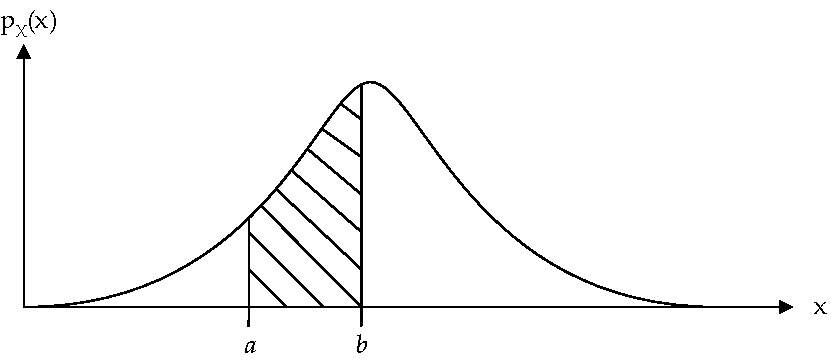
\includegraphics[width=3.5in,height=1.53in]{./image10}
\caption{ A probability density function. The area under the
curve represents the probability that the random variable $X$ lies
in the interval $[ a,b ]$}.
\label{figure:probabilityDensityFunction}
\end{figure}

Let's examine a few more important properties of probability density
functions. The first, which is analogous to
equation~\ref{equ:totalProbabilityEqualOne}, indicates that the
probability of the event space occurring is equal to one. This is known
as the normalization property and it is expressed as

\begin{equation}
\label{equ:integralPDFequals1}
\int^{\infty}_{-\infty} p_x(x)dx = 1
\end{equation}

Another interesting result is obtained by trying to determine the
probability that a random variable takes on an exact value, for example
$P(X=a)$. That is determined from the
integral

\begin{equation}
\label{equ:integralSliceOfPDFequals0}
P(X=a) = \int^{a}_{a} p_x(x)dx = 0
\end{equation}

This is a somewhat counterintuitive result---it indicates that the
probability a random variable can take on a particular value is zero.
Does this make any sense? Consider an experiment where the objective is
to measure a voltage value for a random variable $V$. Now consider
the question, ``\emph{What is the probability that the result of a
voltage measurement equals $\pi$ (the irrational number) volts?}'' In
practice, this question is impossible to answer because the precision
required of the meter is infinite and contrary to its construction. So
the mathematical and practical results are in harmony. There is a way
around this dilemma, which is to determine the probability that the
random variable is within a small range about the target value as
follows

\begin{equation}
\label{equ:integralDeltaSliceOfPDF}
P(\pi < V < \pi+\Delta v) = \int^{\pi+\Delta v}_{\pi} p_V dv \approx p_V(\pi) \Delta v
\end{equation}

This means that the probability a random variable is within a small
range about a given value is approximated by the product of the PDF
evaluated at the value and the size of the range.

\subsection{Mean and Variance}
\label{subsection:mean-and-variance}

Two useful and well-known statistics that are determined from the PDF
are the mean ($\mu$) and variance ($\sigma^2$). 
They are found from the PDF as follows

\begin{equation}
\label{equ:integralDeltaSliceOfPDF}
\mu_x = \int^{\infty}_{-\infty}xp_X(x)dx
\end{equation}

\begin{equation}
\label{equ:integralDeltaSliceOfPDF}
\sigma^2_x = \int^{\infty}_{-\infty}(x-\mu)^2 p_X(x)dx
\end{equation}

The \emph{mean} is analogous to the center of mass of the PDF; it is
also known as the average value. The \emph{variance} is the average of
the squared difference between the mean and the values of the PDF, where
the squared term ensures that a positive difference is taken. The square
root of the variance is known as the standard deviation $\sigma$.

\subsection{Common Probability Density Functions}
\label{subsection:common-probability-density-functions}

There are many PDFs available for describing the seemingly random
variations in the behavior of observed systems and phenomena. In this
section, three common PDFs (normal, exponential, and uniform) are
presented.

\subsection*{The Normal Density}
\label{subsection:the-normal-density}


The most common density function encountered in the physical sciences
and engineering is the normal density. Many population
variations can be described by a normal density. For example, the
resistance values of a large batch of 2.2k ohm resistors would likely
follow a normal density. The normal density is defined as

\begin{equation}
\label{equ:normalDensity}
p_X(x) = \frac{1}{\sqrt{2\pi\sigma}} e^1\frac{1}{2} \ frac{(x-\mu)^2}{\sigma}
\end{equation}

The mean, $\mu$, and standard deviation, $\sigma$, are part of the
definition of the PDF and used to alter the shape of the density to suit
the particular need. The normal PDF is plotted in 
Figure~\ref{figure:normalDensityFunction}. Varying
$\mu$ allows the overall function to be shifted along the x-axis,
while increasing $\sigma$ spreads (or flattens) the function out.
Calculating probabilities from the normal density can be done (although
it takes a bit of work mathematically) so they are usually computed from
something known as the Cumulative Distribution Function that is
presented shortly.

\begin{figure}

\includegraphics[width=2.92708in,height=1.36458in]{./image21}
\caption{A normal density function with the mean ($\mu$)
and standard deviation ($\sigma$) shown.}
\label{figure:normalDensityFunction}
\end{figure}


\subsection*{The Uniform Density}
\label{subsection:the-uniform-density}


The uniform density, plotted in 
Figure~\ref{figure:normalDensityFunction}, models the outcome of an
experiment where all outcomes are equally likely. Mathematically, the
PDF for a uniform density is given by

\begin{equation}
\label{equ:uniformDensity}
p_X(x) = \frac{1}{b-a}, a \leq x \leq b,
\end{equation}

where $a$, $b$ are selected to meet the demands of a particular problem.


\begin{figure}
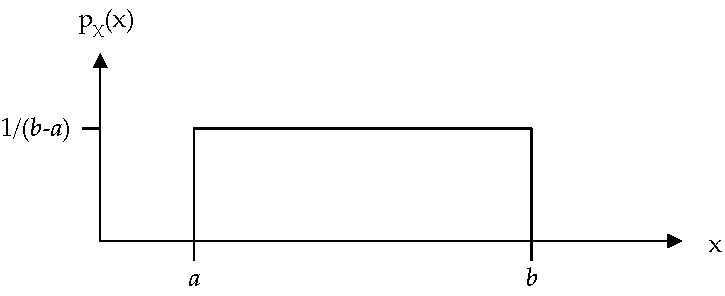
\includegraphics[width=3in,height=1.23in]{./image23}
\caption{The uniform density on the interval $[ a,b ]$.}
\label{figure:uniformDensityFunction}
\end{figure}


\subsection*{The Exponential Density}
\label{subsection:the-exponential-density}


Exponential densities are often utilized to model time dependent
functions, such as inter-arrival times between data packets in
communication systems. As shown later, the exponential density also
describes the behavior of component failures as a function of time. The
mathematical description of an exponential density is

\begin{equation}
\label{equ:exponentialDensity}
p_X(x) = \lambda e^{-\lambda x} , x \geq 0, \lambda \geq 0.
\end{equation}

The PDF is characterized by the parameter $\lambda$ which affects the
shape of the curve as demonstrated in 
Figure~\ref{figure:exponentialDensityFunction}.


\begin{figure}

\includegraphics[width=3in,height=2.1in]{./image25}
\caption{The exponential density for two different $\lambda$ values.}
\label{figure:exponentialDensityFunction}
\end{figure}


\subsection{Cumulative Distribution Functions}
\label{cumulative-distribution-functions}

An important class of questions can be phrased as, ``\emph{What is the
probability that a random variable $X$ is less than value a?"} For
example, the objective might be to determine the probability that an
electronic component will malfunction within two years. Returning to the
first question, it is clear that the goal is to determine the
probability $P(X<a)$, which is found by
integrating the PDF. This result is generalized by allowing the upper
limit of integration to take on an arbitrary value that spans the range
of the random variable. This produces a new function, known as the
\emph{Cumulative Distribution Function} (CDF), which is the integral
function of the PDF and is defined as

\begin{equation}
\label{equ:exponentialDensity}
CDF(x) = \int^x_{-\infty} p_X(y)dy.
\end{equation}

\section{Reliability Prediction}
\label{section:reliability-prediction}

Our main interest in the study of probability stems from the desire to
quantify the reliability of a system. The following is a formal
mathematical definition of \emph{\textbf{reliability}}.

\begin{itquote}
\textbf{Definition}: Reliability, $R(t)$, is the probability that a
device is functioning properly (has not failed) at time $t$.
\end{itquote}

In order to determine $R(t)$, it is necessary to first introduce
some related mathematical entities and their meanings. The
\emph{\textbf{failure rate}}, $\lambda(t)$, of a device is the expected
number of failures per unit time. The failure rate is measured by
operating a batch of devices for a given time interval and noting how
many fail during that interval. A typical graph of failure rate versus
time has the bathtub shape shown in Figure~\ref{figure:bathtubFunction}. 
The high initial failure
rate is a result of manufacturing defects often referred to as infant
mortality. Consequently, many manufactures will ``burn-in'' devices at
the factory, so that if they fail, they do so before being sold. After
the infant mortality phase, devices enter a phase of constant failure
rate, where $\lambda(t) = \lambda$, known as the service life. Estimates for
$\lambda$ are determined empirically by testing a large number of
components. They are usually expressed as a unit failure per a given
number of hours, for example $\lambda  = failure/10^6 hours$.
After some period of time, devices start to wear-out and the failure
rate increases. This usually happens as a result of mechanical wearing
with age and use. Properly designed electronic devices will not have a
wear-out region, instead continuing on at a constant failure rate. This
applies only to the electronic devices themselves, not necessarily to
complete systems that will likely contain mechanical devices.

\begin{figure}

\includegraphics[width=5.5in,height=1.7in]{./image29}
\caption{Failure rate as a function of time, also known as
the bathtub curve.}
\label{figure:bathtubFunction}
\end{figure}

In addition to failure rate, a PDF for the \emph{failure time} of the
device, $f_T(t)$ is defined, where the
random variable is time $T$. This function allows the question to
be asked ``\emph{What is the probability that a device will fail between
time $t_1$ and $t_2$?}'' It is important to
note the difference between $\lambda(t)$ and
$f_T(t)$. The failure rate tells us the
average rate that a collection of identical devices will fail at a given
time $t$, while $f_T(t)$ is a PDF
used to determine the probability that a given device will fail within a
specified time period. A CDF for $f_T(t)$
is determined as



$F(t)$ answers the question ``\emph{What is the probability that
the device has failed by time t?}'' and it is also known as the
\emph{\textbf{failure function}}. Take a few seconds to go back and
review the definition of $R(t)$. It is clear that $R(t)$ is
directly related to $F(t)$ and is its complement. The relationship
between the two is

\begin{equation}
\label{equ:integralDeltaSliceOfPDF}
R(t) = 1 - F(t)
\end{equation}


Since $F(t)$ is a CDF, it increases monotonically from an initial
value of 0 to a maximum value of 1 as time goes to $\infty$ as shown in Figure
8.7. Conversely, $R(t)$ starts at a value of 1 at time zero and
decreases monotonically to a value of 0.


\begin{figure}

\includegraphics[width=2.76in,height=1.56in]{./image33}
\caption{Example reliability and failure functions.}
\label{figure:reliabilityAndFailure}
\end{figure}

Since $\lambda(t)$ represents data that is measured empirically, it is
useful to establish a relationship between $\lambda(t)$ and the ultimate
goal of reliability, $R(t)$. To do so, a relationship between
$\lambda(t)$, $R(t)$, and  is
established as follows. Consider a small period of time between $t$
and $\Delta 4$, and determine the
probability of device failure during this period. From the approximation
developed in 
equation~\ref{equ:integralDeltaSliceOfPDF}, this probability is given by

\begin{equation}
\label{equ:failureBetweenUsingT}
P(failure between t and \Delta t) \approx f_T(t) \Delta t
\end{equation}

How is this probability related to $R(t)$ and $\lambda(t)$?
$R(t)$ provides the probability that the device is working at time $t$
and $\lambda(t)$ gives the probability that the device will fail
at time $t$. The product of $R(t), \lambda(t)$, and $\Delta t$ gives
the same probability of failure in equation~\ref{equ:failureBetweenUsingT}.

\begin{equation}
\label{equ:failureBetweenUsingR}
P(failure between t and \Delta t) \approx R(t) \lambda(t) \Delta t
\end{equation}

Setting equations~\ref{equ:failureBetweenUsingT} and  {equ:failureBetweenUsingR} 
provides the desired relationship between the three quantities

\begin{equation}
\label{equ:failureBetweenUsingR}
f_T(t) = R(t) \lambda(t) ,
\end{equation}

that is fundamental in establishing the connection between $R(t)$
and $\lambda(t)$. However, the PDF $f_T(t)$ needs to be eliminated 
from equation~\ref{equ:failureBetweenUsingR}. This is accomplished 
through its relationship to the CDF
$F(t)$, and thus $R(t)$, as follows

\begin{equation}
\label{equ:cdfOfF}
f_T(t) = \frac{d}{dt}F(t) = \frac{d}{dt}\big[1-R(t)\big] = -\frac{d}{dt}R(t)
\end{equation}

Equating this result with equation~\ref{equ:failureBetweenUsingR}
produces

\begin{equation}
\label{equ:cdfOfF}
f_T(t) = \frac{d}{dt}F(t) = \frac{d}{dt}\big[1-R(t)\big] = -\frac{d}{dt}R(t)
\end{equation}

Integrating both sides gives

\begin{equation}
\label{equ:bigIntegral}
\int^{t}_0 \big[  \frac{ - \frac{d}{dt}}{R(\tau)} R(\tau) \big] \delta \tau = \int^t_0 \lambda(\tau) \delta \tau \Rightarrow -ln(R(t)) = \int^t_0\lambda(\tau)\delta \tau
\end{equation}

and solving for $R(t)$ produces the final result for reliability as
a function of $\lambda(t)$ 

\begin{equation}
\label{equ:rAsFunctionOfLambda}
R(t) = exp \big[ - \int^t_0\lambda(\tau)\delta \tau \big]
\end{equation}

During the service lifetime phase, the failure rate is constant, which
simplifies to

\begin{equation}
\label{equ:rAsFailureConstant}
R(t) = exp (- \lambda(t))
\end{equation}

This important result is now applied in Example 8.1.

\begin{table}
\begin{tabular}{m{15cm}||}
\textbf{\hfill\break{Example 8.1}}
Transistor Reliability

\emph{\textbf{\ul{Problem:}}} Consider a transistor with a constant
failure rate of $\lambda = 1/10^6 hours$. What is the
probability that the transistor will be operable in 5 years? \\

\emph{\textbf{\ul{Solution:}}} This solution is found using the
reliability function for a constant failure rate in 
equation~\ref{equ:rAsFailureConstant} as follows.

$$R(t) = exp(-\lambda t)  $$\\
$$R(5 years) = exp\big( - \frac{1}{10^6 hours} x \frac{24 hours}{day} X \frac{365 days}{year} X 5 years \big) = $$\\
$$			= exp(-0.0438) $$ \\
$$			= 0.957 $$\\
$$			= 95.6 \% $$
\end{tabular}
\end{table}

\subsection{Mean Time to Failure}
\label{subsection:mean-time-to-failure}

The \emph{\textbf{mean time to failure}} (MTTF) is a quantity which
answers the question, ``\emph{On average how long does it take for a
device to fail?}'' From its definition, it is apparent that the MTTF is
the mean value of the random variable $T$ (failure time). It is
determined from the PDF and the definition of the mean in (8) as follows

\begin{equation}
\label{equ:mttfIntegral}
MTTF = \int^\infty_0 t f_T(t) dt 
\end{equation}

At this point the form of the PDF for $f_T(t)$ is not known, but it can be
found from equation~\ref{equ:cdfOfF} since it is the negative derivative 
of $R(t)$. Assuming the form of $R(t)$ found in 
equation~\ref{equ:rAsFailureConstant} for a constant failure rate gives

\begin{equation}
\label{equ:mttfConstantFailureRate}
f_T(t) = -\frac{d}{dt}R(t) = \lambda e^{-\lambda t}
\end{equation}

This means that under the condition of a constant failure rate, the
failure PDF follows an exponential density. The MTTF is found from
$f_T(t)$ via integration by parts to be

\begin{equation}
\label{equ:mttfConstantFailureRate}
MTTS = -\int^\infty_0 t e^{-\lambda t} = \frac{1}{\lambda}
\end{equation}

This makes intuitive sense because $\lambda$ is the expected number of
failures per unit time for a device. Consequently, the reciprocal of
$\lambda$ is the expected time between failures or MTTF. Let's consider a
few examples.

\begin{table}
\begin{tabular}{m{15cm}||}
\textbf{\hfill\break{Example 8.2}}
Transistor MTTF\\

\emph{\textbf{\ul{Problem:}}} Consider the transistor in Example 8.1.
(a) Determine the MTTF, and (b) the reliability at the MTTF.

\emph{\textbf{\ul{Solution:}}}

(a) From equation~\ref{equ:mttfConstantFailureRate} the 
$$MTTF =\frac{1}{\lambda} = \frac{1}{1/10^6 hours} = 10^6 hours $$\\
$$		= 114 years $$.\\

(b) From equation~\ref{equ:rAsFailureConstant} the reliability at 114 years is

$$R(t) = exp(-\lambda t) $$\\
$$	R(114 years) = exp\big( -\frac{10^6 hours}{10^6 hours}\big) = exp(-1) = 0.368 $$\\
$$	= 36.8\%$$.
\end{tabular}
\end{table}

This is a bit counterintuitive. Although the average time between
transistor failures is 114 years, an individual transistor has only a
36.8\% chance of surviving to 114 years. It would seem logical that the
reliability at 114 years should be 50\% and that the transistor would
have a 50-50 chance of failing. This would be true if $f_T(t)$
were symmetric about its mean,
but that is not the case for the exponential density.

\begin{table}
\begin{tabular}{m{15cm}||}
\textbf{\hfill\break{Example 8.3}}
Human lifespan estimation.\\

\emph{\textbf{\ul{Problem:}}} Data shows that for a 30 year old
population, the failure (death) rate is constant with approximately 1.1
deaths per 1000 people per year. Given this data, estimate the MTTF of
humans.

\emph{\textbf{\ul{Solution:}}} In order to find MTTF, $\lambda$ is 
needed. From the information given it is

$$\lambda = \frac{(1.1/1000) failures}{1 year} = \frac{1.1 failure}{10^3 years}=\frac{1 failure}{909 years}$$

From this MTTF is computed as

$$MTTF  = \frac{1}{\lambda} = 909 years!$$

\end {tabular}
\end{table}


While great news for those of us seeking longevity, this calculation is
clearly wrong since the upper limit on human lifespan is empirically
known to be about 120 years. Why is this so? Serious problems arise if
$R(t)$ is used in situations where the underlying assumption is
invalid. The results in equations~\ref{equ:rAsFailureConstant} and 
\ref{equ:mttfConstantFailureRate} apply only if the failure rate is
constant. Although that is nearly true for people in their 20s and 30s,
it is not true as people age. People do wear out and the failure rate
increases with age.

\subsection{Failure Rate Estimates}
\label{subsection:failure-rate-estimates}

The overriding objective of this chapter is to estimate the future
behavior of devices that are used in electrical and computer systems.
The particular behavior of interest is the state of a device's
functionality---the reliability, is it working or has it failed?
Equation (23) indicates that it is fairly straightforward to determine
reliability, if the failure rate ($\lambda$) is known and is constant.
One question to consider is what factors influence the failure rate of a
device. Many of us probably have had experiences in the laboratory where
we have caused devices to fail by subjecting them to conditions outside
of the normal operating bounds, notably excessive current, power, or
heat. In those cases the devices probably failed, or burned up, due to
the operating conditions outside of the allowed bounds for the device.
However, even when operated within the allowable norms of a device's
operating conditions, variations in factors such as power, operating
voltages, and temperatures impact $\lambda$.

The United States Military has kept copious records of device failures
in the field and the conditions under which they operated. These records
are synthesized in a handbook entitled \ul{Reliability Prediction of
Electronic Equipment} {[}MIL-HDBK-217F{]} that provides failure rates
for various analog and digital components, along with adjustment factors
to account for operating conditions, the environment, and device
quality. Categories of devices included in the handbook are switches,
fuses, diodes, optoelectronic devices, and microelectronic devices (op
amps, logic devices, microcontrollers, microprocessors). The handbook
was last published in 1991 and has been discontinued, but it is still
widely accepted and used. Bellcore (subsequently Telcordia) has
developed newer models {[}Tel96{]} based upon MIL-HDBK-217F that were
updated to better predict the reliability of components. MIL-HDBK-217F
is used here since it is freely available in the public domain.

Failure rates for resistors, capacitors, transistors, and integrated
circuits from MIL-HDBK-217F are included in Appendix C. For each device,
a base failure rate is given, $\lambda_b$, and multiplied
by a number of adjustment factors, denoted by the symbol
$\pi$, to estimate the device failure
rate $\lambda$. Each adjustment factor has a unique subscript and their
values are found from tables or equations in the handbook.

For example, consider the low frequency field effect transistor in
Appendix C. The overall failure rate is given by the equation
$\lambda=\lambda_b \pi_tau \pi_A \pi_Q \pi_E failures /10^6 hours$.
$\lambda_b$  is the base failure rate that is directly read from a table, 
 $\pi_\tau$ is a temperature factor which is computed from an 
 exponential equation (be careful to use the junction temperature 
 as indicated in Appendix C),
$\pi_A$ is an application factor that depends upon how the device 
will be used, $\pi_Q$ is a quality factor, and $\pi_E$ is an 
environmental factor. The
quality factor table lists some strange names and values from 0.7 to
8.0. The quality factor describes the level of burn-in and screening
each device receives before leaving the factory. Joint Army/Navy (JAN,
JANTX, and JANTXV) quality factors are the highest standard, and are
usually required only for space vehicles. That individual attention to
burn-in means that JAN parts are expensive and most JAN devices have
passed their infant mortality phase before leaving the factory. When
determining failure rate for a device from a table, it is common
practice to always round parameters or values pessimistically so that
the evaluation is a worst case analysis of its performance. That way the
device should perform with a higher reliability when embedded into a
system, hopefully causing only pleasant surprises in operation. Finally,
the factor $\pi_E$ is based upon the
different operating environments that are identified in Appendix C.
Example 8.4 demonstrates the application of the MIL-HDBK-217F standard
for reliability estimation.

In summary, it is possible to estimate the reliability of devices if the
failure rate is known and it is constant. The US Military and Telecordia
handbooks provide guidance for estimating failure rates, and thus the
component reliability. It must be kept in mind that they are estimates
and not guaranteed to predict the exact performance. It is also apparent
that this can become a rather time-consuming process if there are many
components in a system, and thus the use of reliability software
packages may be warranted.

\begin{table}
\begin{tabular}{m{15cm}|}
\textbf{\hfill\break Example 8.4}
Reliability estimation using the MIL-HDBK 217F. \\

\emph{\textbf{\ul{Problem:}}} Consider the circuit below that contains a
bipolar junction transistor (BJT). This electronic circuit is a simple
digital logic inverter. When the input voltage $V_I$ is 0, 
the BJT is off, no current
flows through any branches of the device, and the output voltage,
$V_O$, is 5V. When the input is 5V
(high) the BJT goes into saturation due to the high base current (low
$R_B$), producing a 50mA collector
current, a large voltage drop across $R_C$, and an output
voltage close to 0V. The average collector current for the two states is
25mA, producing an average power of 125mW (25mA×5V). Assume that the
circuit is used in a missile launcher, the ambient temperature is 25°C,
and that JANTX quality parts are used. Determine the MTTF and
reliability for the 2N3904 BJT (a low power, low frequency BJT) in 20
years.

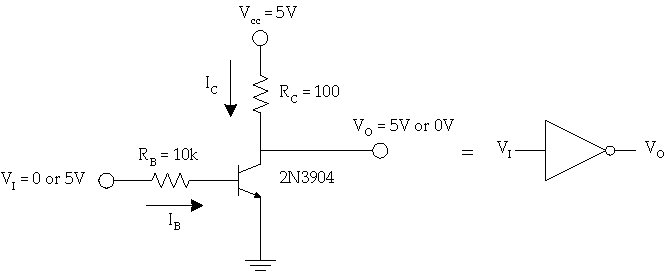
\includegraphics[width=4.25in,height=1.74in]{./image63}


\emph{\textbf{\ul{Solution:}}} The objective of this problem is to
determine the failure rate, from which the MTTF and reliability are
estimated. From the MIL-HDBK-217F data in Appendix C, the failure rate
is


$$\lambda=\lambda_b \pi_tau \pi_A \pi_R \pi_S \pi_Q \pi_E \frac{failures}{10^6 hours}$$


The base failure rate is given directly as
$\lambda_b = 0.00074$.   $\pi_\tau$ is the temperature factor and
its value is determined from the relationship

$$\pi_\tau = exp \big[-2114 \big[ \frac{1}{T_j + 273} - \frac{1}{298} \big] \big]$$

where $T_j$ is the junction temperature. As
indicated in Appendix C, it is computed as

$$T_j = T_A + \Theta_{jA}P_D = $$ \\
$$		25^\circ C \big( 200 \frac{^\circ C}{W} \big) \big(125 X 10^{-3}W \big) = 50^\circ C $$

The thermal resistance, $\Theta_JA$, is read
from the 2N3904 datasheet (Appendix D) and will be examined in more
detail shortly. The temperature factor is

$$\pi_\tau = exp \big[-2114 \big[ \frac{1}{50 + 273} - \frac{1}{298} \big] \big] = 1.73$$

$\pi_A$ is an application factor
(switched or linear amplification), and the value for the switched logic
inverter is $\pi_A = 0.70$.  $\pi_R$ is a power rating factor that is
computed based upon the maximum rated power dissipation of the 2N3904
(625mW from the component datasheet in Appendix D) as follows:
$$\pi_R = P_R^{0.37} = 0.625^{0.37} = 0.84$$


$\pi_S$ is a stress factor that is
computed from the ratio of the maximum collector-emitter voltage over
the maximum rated value of the device. In this circuit, the maximum
value of $V_{CE}$ is 5V (when the device
is off and no current flows), while the maximum rated value of
$V_{CE}$ from the 2N3904 datasheet is 40V.

$V_S = \frac{applied V_{CE}}{rated V_{CE}} = \frac{5}{40} = 0.225$

$\pi_Q$ is the quality factor, and based upon the fact that a JANTX part is 
$\pi_Q = 1.0$.  $\pi_E$ is the environmental factor, and
for the missile launch application, $\pi_E = 32.0$.

All of this is brought together to compute the failure rate. The product
of the adjustment factors is computed as

$$\lambda=\lambda_b \pi_tau \pi_A \pi_R \pi_S \pi_Q \pi_E \frac{failures}{10^6 hours} = $$\\
$$	= \big( \frac{7.4x10^{-4}}{10^6 hours} (1.73)(0.7)(0.84)(0.066)(1.0)(32.0) \big) $$\\
$$	= \frac{1.59x10^{-3} failures}{10^6 hours}$$

This allows estimation of the MTTF and requested reliability
$$	MTTF = \frac{1}{\lambda} = 6.3x10^8 hours = 71,804 years. $$\\
$$	R(20 years) = exp \big( -\frac{20 years}{71,804 years} \big) = 0.9997 $$\\
$$	= 99.97\%$$

In conclusion, the BJT is estimated to be highly reliable in 20 years.

\end{tabular}
\end{table}



\subsection{Thermal Management and Power Derating}
\label{subsection:thermal-management-and-power-derating}

One of the quantities computed in Example 8.4 was the junction
temperature, $T_J$, which was computed from the
power dissipated in the device and a quantity known as thermal
resistance, $\theta$. It is important to understand this in more detail,
since it impacts the reliability of microelectronic devices.
Furthermore, if the junction temperature exceeds a certain value, the
device will fail. Thus, thermal management issues need to be taken into
account. We start with a physical model in Figure 8.8 (a), which has a
junction (the integrated circuit or device), enclosed by a case (the
packaging of the device), surrounded by ambient environmental
conditions. In part (b) a heat sink is included which aids in thermal
transfer. Each element has associated with it a quantity known as
thermal resistance that measures the ability of that particular element
to transfer heat to another element. A result from heat transfer for
electronics is that changes in temperature ($\Delta T$) are proportional
to the product of power dissipation ($P_D$) and the thermal resistance.
This relationship is

\begin{equation}
\label{equ:thermalHeatFlow}
\Delta T = P_D \Theta
\end{equation}

It is similar to Ohm's Law where the change in temperature, power, and
thermal resistance (units = °C/W) are analogous to voltage, current, and
electrical resistance respectively. The total thermal resistance between
two elements, such as between ambient and the junction, is the sum of
all thermal resistances between them. In the case with no heat sink,
this produces a junction to ambient resistance of
$\Theta_{JA} =  \Theta_{JC} + \Theta_{CA}$, while in the case with a heat
sink, 
$\Theta_{JA} = \Theta_{JC} + \Theta_{CA} + \Theta_{SA}$. In the case 
of the heat sink, $\Theta_{CA}$ is replaced by the sum
$\Theta_{CS} + \Theta_{SA}$, which has a lower combined
thermal resistance and greater ability to dissipate heat.

\begin{figure}
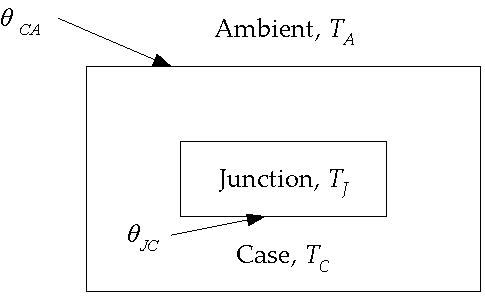
\includegraphics[width=2.1in,height=1.3in]{./image91}

\includegraphics[width=3in,height=1.56in]{./image92}
\caption{Physical model of microelectronic devices with
thermal junctions and temperatures indicated. (a) Device inside casing.
(b) Device inside casing with a heat sink added.}
\label{figure:thermalModelsBJT}
\end{figure}

This Ohm's Law type of relationship means that thermal transfer can be
modeled using familiar resistive circuits as shown in 
Figure~\ref{figure:thermalModelAsCircuit}. Based
upon this circuit model, the temperature can be found at different
points from the thermal resistance and power dissipation. Most
importantly the junction temperature is found as

\begin{equation}
\label{equ:thermalHeatFlow}
T_J = T_A + P_D \Theta_{JA}
\end{equation}

\begin{figure}
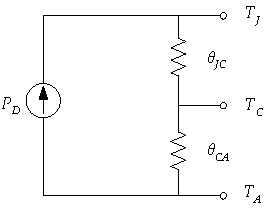
\includegraphics[width=1.84in,height=1.49in]{./image94}
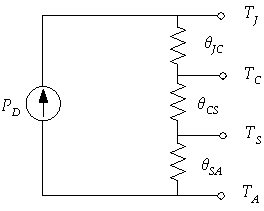
\includegraphics[width=1.8in,height=1.48in]{./image95}
\caption{Resistive models for thermal transfer in
microelectronic devices. (a) Device with no heat sink. (b) Device with a
heat sink added.}
\label{figure:thermalModelAsCircuit}
\end{figure}

Let's now apply these results. Manufacturer datasheets typically
identify the absolute maximum power dissipation and note that the device
should be derated if operated at ambient conditions above room
temperature ($T_A = 25^circ C$). The datasheets
also supply a maximum junction temperature for the device. It is clear
from the resistive model that, for a fixed power dissipation, the
junction temperature increases along with ambient temperature. If the
maximum junction temperature is exceeded, the device will be destroyed.
Another way to look at this is that as ambient temperature increases,
the maximum amount of power a device can dissipate decreases. This
decrease in maximum power dissipation is known as
\emph{\textbf{derating}}. From equation~\ref{equ:thermalHeatFlow}
 the maximum power that can be
dissipated in a device at a given ambient temperature is

\begin{equation}
\label{equ:powerFunctionTemperature}
P_{D,max} = \frac{T_{J,max}  - T_A}{\Theta_{JA}}
\end{equation}

From this relationship, a power derating curve is plotted in 
Figure~\ref{figure:typicalDeratingCurve}
showing the maximum power versus ambient temperature. Example 8.5
demonstrates the application of this to the inverter in Example 8.4.

\begin{figure}
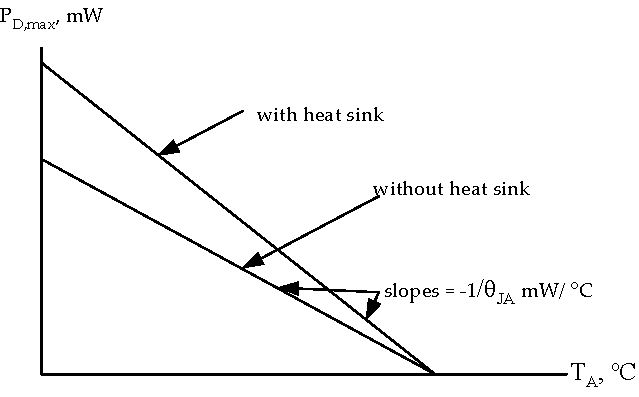
\includegraphics[width=3.36in,height=2.1in]{./image98}
\caption{Typical power derating curves.}
\label{figure:typicalDeratingCurve}
\end{figure}

\begin{table}
\begin{tabular}{m{15cm}|}
\textbf{Example 8.5} 
Power Derating for the Inverter Circuit.\\

\emph{\textbf{\ul{Problem:}}} Assume the circuit in Example 8.4 is
operating at an ambient temperature $T_A = 120^\circ C$ and 
that no heat sink is used.
(a) Determine the derated power and if the design is within the
manufacturer's limits for power dissipation at this temperature and, (b)
re-compute the reliability at 20 years based upon this elevated
operating temperature.

\emph{\textbf{\ul{Solution:}}}
(a) From the manufacturer datasheet in Appendix D, the 2N3904 BJT has a
thermal resistance of $\Theta_{JA} = 200^\circ C/W$ and a
maximum junction temperature of 150°C. From this the maximum power is
computed from equation~\ref{figure:typicalDeratingCurve} as

$$P_{D,max} = \frac{(150 - 120)^\circ C}{200^\circ C/W} = 150mW$$

The derated, or maximum, power at this temperature is \ul{150mW}.
Clearly, the 125mW of power dissipated as determined in Example 8.4 for
the BJT is within this derated limit.

(b) To compute the failure rate the junction temperature and
$\pi_\tau$ are re-computed.

$$T_J = T_A + P_D\Theta_{JA} = 120^\circ C + (125x10^{-3} W) \big[ \frac{200^\circ C}{W} \big]= 145\circ C $$\\
$$\pi_T = exp\big[ -2114 \big[ \frac{1}{145+273} - \frac{1}{298} \big] \big] = 7.66$$
\end{tabular}
\end{table}

With this new value, the value of $\lambda=7.00x10^{-3}/10^6 hours$, and 
the reliability is reduced slightly to \ul{99.88\%}. Note, however, the junction 
temperature is
quite high at 145°C and further increases in temperature would likely
destroy the device.

\subsection{Limits of Reliability Estimation}
\label{subsection:limits-of-reliability-estimation}

It must be kept in mind that the reliability estimates are just that,
estimates, and there are limitations in their use. First, realize that
the failure rate data comes from accelerated stress tests, where devices
are put under stress beyond normal operating conditions, and from these
the failure rates are estimated. (Nobody sits around waiting 20 years
for the devices to fail!) The tests are based upon mathematical models
for the failure rate and the device lifetime. Secondly, there are other
factors that influence reliability that are not addressed by $\lambda$,
such as the manufacturing processes used, the quality of manufacturing
technologies, shock, and corrosion. Part of the value of reliability
estimation is for comparative purposes when evaluating different design
options. Applying these methods forces the designer to consider the
operating conditions and factor them into the design.

\section{System Reliability}
\label{section:system-reliability-1}

The previous section focused on determining the reliability of a single
device. It is natural to ask, ``\emph{How can the reliability of a
system consisting of many devices be determined?}'' In order to derive
the overall reliability of a multi-component system, it is necessary to
take into account the overall system structure.

\subsection{Series Systems}
\label{subsection:series-systems}

Consider the inverter circuit in Example 8.4---failure of any one
component in the circuit would lead to the failure of the overall system
or circuit. Conceptually, a system in which the failure of a single
component (or subsystem) leads to failure of the overall system is known
as a \emph{\textbf{series system}}. Figure~\ref{figure:seriesSystems}
shows a block diagram of a series system composed of boxes
$S_1, S_2, \ldots S_n$ that represent the components,
or the subsystems, of a larger system.

\begin{figure}
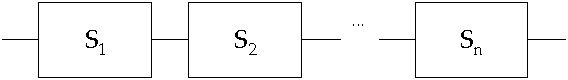
\includegraphics[width=3.21in,height=0.45in]{./image109}
\caption{A series system consisting of components, or subsystems $S_1, S_2, \ldots S_n$.}
\label{figure:seriesSystems}
\end{figure}

To compute the overall reliability of a series system, $R_s(t)$, 
it is assumed that the failure
of subsystems or components are independent events. The system is
operable only if subsystems $S_1 and S_2 \ldots S_n$ are all simultaneously
operating. Therefore, the probability of the overall system operating is
given by the product of reliabilities for all of the subsystems as
follows

\begin{equation}
\label{equ:seriesProbability}
R_s(t) = R_1(t)R_2(t)\ldots R_n(t) = \prod_{i=1}^n R_i(t) 
\end{equation}

It is important to remember that failures are assumed to be independent
events, just as flipping a coin twice is considered two independent
events. The overall system reliability is less than or equal to that of
any single subsystem, since all reliability values are $\leq 1$. Thus
$R_s$ decreases as the number of
subsystems increases. Assuming a constant failure rate for all system
components gives the following result for the overall system reliability

\begin{equation}
\label{equ:seriesProbabilityConstantErrorRate}
R_s(t) = e^{-\lambda_1t}e^{-\lambda_2t}\cdots e^{-\lambda_nt} = exp(-\sum_{i-1}^n \lambda_i t
\end{equation}

This leads to a series system failure rate and MTTF of


\begin{equation}
\label{equ:seriesProbabilityMttf}
\lambda_s = \sum_{i=1}^n \lambda_i
MTTF = \frac{1}{\lambda_s}
\end{equation}

Example 8.6 revisits the inverter problem where the failure rates of all
components are considered for system reliability estimation.


\begin{table}
\caption{}
\label{table:<context>}
\begin{tabular}{|m{15cm}|}
\textbf{\hfill\break Example 8.6} 
Inverter circuit reliability.

\emph{\textbf{\ul{Problem:}}} For the system in Example 8.4 estimate (a)
the overall system reliability in 20 years, and (b) the MTTF. Assume
room temperature and that ¼ watt fixed composition resistors are used.

\emph{\textbf{\ul{Solution:}}}

(a) Conceptually this is a series system---if any of the individual
components fail, then the overall system will fail. That means that
failure rates for the two resistors are needed in addition to the value
previously computed for the transistor. They depend upon the power
dissipated in each resistor, which is 125mW and 0.9mW for the collector
and base resistors respectively. The failure rate for a fixed
composition resistor from MIL-HDBK-217F is

$$\lambda_{resistor1} = \lambda_b \pi_R \pi_Q \pi_E failures/10^6 hours$$

For the collector resistor, $R_C$, the base failure rate is
computed as

$$ \lambda_b = 4.5x10^{-9} exp \big[ 12 \big[\frac{T+273}{343} \big] \big] exp\big[ \frac{S}{0.6} \ frac{T+273}{273}\big] \big]$$
$$  = 4.5x10^{-9} exp \big[ 12 \big[\frac{25+273}{343} \big] \big] exp\big[ \frac{0.125/0.25}{0.6} \ frac{25+273}{273}\big] \big]$$
$$ = 3.77x10^{-4}$$

The $S$ term is the ratio of power dissipated to the maximum power
rating. The values $\pi_R=1.0$, $\pi_Q=15.0$, and $\pi_E = 27.0$ 
are directly read from tables.
Thus the overall failure rate for the collector resistor is

$$\lambda{resistor2} = (3.77x10^{-4}(1.0)(15.0)(27.0) = 1.53x10^{-1} failure/10^6 hours$$

The process for the base resistor, $R_B$, is similar, and results in

$$\lambda{resistor2} = 6.1x10^{-2} failure/10^6 hours$$

The total failure rate is given from equation~\ref{equ:seriesProbabilityMttf} as

$$\lambda_s = \lambda_{BJT} + \lambda{resistor1} + \lambda{resistor2} = 0.215 failures/10^6 hours$$

$$R_s(t) =exp(-\lambda_s t) = exp \big( -\frac{0.215}{10^6 hours} x \frac{24 hours}{day} x \frac{365 days}{year} x 20 years \big)$$
$$96.3 \%$$

Since resistors are pretty reliable devices, the overall system
reliability decreases only a small amount relative to that of the BJT
itself.

(b) The MTTF is given by $1/\lambda_s$ which in this case is \ul{531 years}.
\end{tabular}
\end{table}



\subsection{Parallel Systems}
\label{subsection:parallel-systems}

From (30) it is clear that as more components are added to a series
system, the reliability decreases. It is natural to ask if the
reliability can be increased. The use of redundancy gives us a method to
answer in the affirmative. A design has \emph{\textbf{redundancy}} if it
contains multiple modules performing the same function where a single
module would suffice. By its very nature redundancy allows improperly
functioning modules to be switched out of the system without affecting
its behavior. With redundancy the overall system functions correctly
when any one of the submodules is functioning. 
Figure~\ref{figure:parallelSystem} shows a
simplified view of a \emph{\textbf{parallel system}} with subsystems
$S_1, S_2, \ldots S_n$.

\begin{figure}
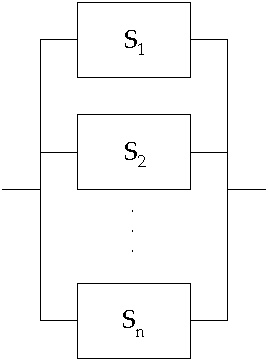
\includegraphics[width=1.5in,height=2in]{./image129}
\caption{A parallel, or redundant, system consisting of
subsystems $S_1, S_2, \ldots S_n$}
\label{figure:parallelSystem}
\end{figure}

In order to compute the reliability of a parallel system, note that a
parallel system functions correctly when $S_1$ is functioning correctly, or
$S_2$ is functioning correctly, $\ldots or S_n$ is functioning
correctly. It would be nice if it were possible to write an equation
stating that 
$R_s(t) = R_1(t) + R_2(t) + \ldots R_n(t)$ where + is
the logical OR operator. Unfortunately, there is no direct way to
realize the OR operation in probability theory. This is resolved by
working with failure function, $F(t)$, instead. The probability
that the system will fail by time $t, F_s(t)$, is equal to the probability
that subsystem $S_1$ will fail and $S_2$ will fail and $\ldots S_n$
will fail. This probability is expressed mathematically as


\begin{equation}
\label{equ:parallelFailureRate}
F_s(T) = F_1(t)F_2(t) \ldots F_n(t) = \prod_{i=1}^nF_i(t) = \prod_{i=1}^n(1-R_i(t))
\end{equation}


The overall system reliability of the parallel system is found from this
as

\begin{equation}
\label{equ:parallelReliability}
R_s(t) = 1-F_S(t) = 1 - \prod_{i=1}^n \big[ 1-R_i(t) \big]
\end{equation}

As more redundant components are added to a parallel system, additional
$1-R_i(t)$ terms are introduced into the
product term. This decreases the value of the product, hence the overall
system reliability is increased as more redundant systems are added.

In order for a parallel system to work, a mechanism must be in place to
monitor each of the subsystems to make sure that they are operating
correctly. Developing circuits to detect failures and control the
switching between subsystems can be complex and is not considered here.
Special care must be paid to the switching circuit itself, as
malfunction of this circuit could lead to an overall system failure. An
example of parallel system reliability is given in Example 8.7.


\begin{table}
\begin{tabular}{m{15cm}|}
\textbf{Example 8.7} 
Reliability of a Redundant Array of Independent Disks (RAID).\\

\emph{\textbf{\ul{Problem:}}} In a RAID, multiple hard drives are used
to store the same data, thus achieving redundancy and increased
reliability. One or more of the disks in the system can fail and the
data can still be recovered. However, if all disks fail, then the data
is lost. For this problem, assume that the individual disk drives have a
failure rate of $\lambda = 10 failuresx/10^6 hours$. How many disks
must the system have to achieve a reliability of 98\% in 10 years?

\emph{\textbf{\ul{Solution:}}} The reliability of a parallel system with
redundancy is given by equation~\ref{equ:parallelReliability}. 
Since all of the disks are identical, the expression simplifies to

$$R_s(t) = 1 - \left[ 1 - R_i(t) \right]^n$$

$$0.98 \leq 1 - \big[ 1 - exp\big( - \frac {10}{10^ hours} x \frac{24 hours}{day} x \frac{365 days}{year} x 10 years \big) \big]^n$$

$$0.98 \leq 1 - \left[1-0.42\right]^n$$

$$0.02 \leq (0.58)^n$$

$$log(0.02) \leq nlog(0.58)$$

$$n \geq 7.2$$
\end{tabular}
\end{table}

In order to achieve this reliability, \ul{n=8} disks are required. The
reliability of each individual disk is low at 42\%, but using
redundancy, the overall system reliability is quite high.

\subsection{Combination Systems}
\label{subsection:combination-systems}

Many real systems do not fit neatly into either parallel or series
reliability models as shown in Figure 8.13. Rather, they may be a
combination of the two, and such systems will be referred to as
combination systems. One way to determine the reliability of a
combination system is to utilize the results obtained for series and
parallel systems in (30) and (34). The system network is reduced by
combining parallel subsystems into a single block, whose reliability is
given by (34), while series subsystems are reduced to a single block
whose reliability is given by (30). This is conceptually analogous to
combining series and parallel resistances in electrical circuits. The
network is continually reduced until only a single block remains whose
reliability is known from all of the subsystem combinations.

To illustrate this, consider the system in Figure 8.13. To determine the
reliability, start by combining the three parallel systems
$S_2, S_3, and S_4$ whose
reliability is determined by application of (34) to be 
$R_{s_{2-4}}(t) = 1- (1-R_2(t))(1-R_3(t))(1-R_4(t)))$.
The result is then combined with $S_1$ in series to give the
overall system reliability, 

$R_{s}(t) = R_1(t) \left[ 1- (1-R_2(t))(1-R_3(t))(1-R_4(t))) \right]$.


\begin{figure}
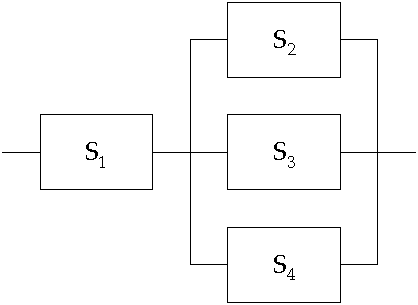
\includegraphics[width=2.35in,height=1.72in]{./image149}
\caption{A combination series-parallel system. $S_2, S_3, and S_4$
are redundant parallel systems.}
\label{figure:}
\end{figure}


The chapter concludes with Example 8.8 that addresses combination system
reliability.


\begin{table}
\caption{}
\label{table:<context>}
\begin{tabular}{m{15cm}|}
\textbf{Example 8.8} 
Combination system reliability. \\

\emph{\textbf{\ul{Problem:}}} Consider the system shown below with the
following reliabilities at a fixed time $t, R_1=R_2= 80\%$. 
Determine the reliability that subsystems $R_3, and R_4$
must have so that the overall system reliability is greater than 95\%.

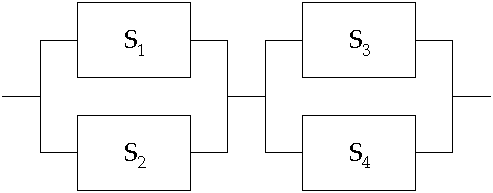
\includegraphics[width=2.8in,height=1.1in]{./image153}

\emph{\textbf{\ul{Solution:}}} The parallel systems can combined into
single systems whose reliabilities are

$$R_{s_{1,2}} = 1 - (1-R_1)(1-R_2) $$

$$R_{s_{3,4}} = 1 - (1-R_3)(1-R_4)$$

They are combined in series to give the overall system reliability

$$R_s = \left[ 1 - (1-R_1)(1-R_2) \right] x \left[ 1 - (1-R_2)(1-R_3) \right]$$

Substituting values and assuming $R_3 = R_4$ gives

$$0.95 = \left[ 1-0.2^2 \right] \left[1 - (1-R_{3,4})^2 \right]$$.

Solving for the reliabilities gives the final result

$$R_3 = R_4 = 0.90$$
\end{tabular}
\end{table}

This example demonstrates the power of redundant systems.
$S_1 and S_2$ have somewhat low reliabilities
relative to the overall system goal, but the reliability of the parallel
combination of $S_1$ and $S_2$ is 96\%. It requires a
reliability for systems 3 and 4 of $R_3 = R_4 = 90\%$, while the combined
reliability of systems 3 and 4 is 99\%.

\section{Summary and Further Reading}
\label{section:summary-and-further-reading}

This chapter presented the basics of probability theory and methods for
estimating the reliability of components and systems. Failure rate is an
important quantity that is determined empirically and provides the rate
of failure over the lifetime of a component or system. A mathematical
definition of reliability was derived from this quantity, which takes a
simple exponential form in the case of a constant failure rate. This was
applied to estimate the reliability of single components, particularly
using failure rates from MIL-HDBK-217F. Issues of thermal transfer and
power derating were considered. Reliability estimation was extended to
more realistic systems consisting of multiple components in series and
parallel forms. The use of redundancy with parallel systems to increase
the overall system reliability was addressed.

There are plenty of good textbooks available on the probability theory,
if it is necessary to study probability theory further. The book
\ul{Practical Reliability of Electronic Equipment and Products}
{[}Hna03{]} provides detailed coverage for electrical systems
reliability. It includes factors not considered here such as thermal
management on printed circuit boards, procurement practices, and
electromagnetic interference. Two excellent articles that demonstrate
the application of design for reliability and redundancy for an embedded
system application are by George Novacek in \ul{Circuit Cellar} magazine
{[}Nov00, Nov01{]}.
